%Start: 22/04/14
%Last edited on 17/09
	%Complete revision after committee meeting and NERD club
	%More straightforward story, clearer results with a more simple measure of diversity, took out the mandibles completely
	%Now aiming for the Journal of Mammalogy (needs very different formatting)


% Preamble
\documentclass[12pt,a4paper]{article}
\usepackage{enumerate} 	% put in numbers or bullet points
\usepackage{setspace}	% line spacing					
\usepackage{authblk}	% For author affiliations
\usepackage{graphicx} 	% For adding pictures

\usepackage[nomarkers]{endfloat} %Figures and tables at the end of the document
\usepackage{pdflscape}	% for landscape pages
\usepackage{mathtools}	% For equations etc.
\usepackage[osf]{mathpazo} % palatino font package
\usepackage{fixltx2e}	% includes subscripts
\usepackage{ms}     	% load the manuscript style template

%\usepackage{float}		% Use these options to have figures in specific places in the text
%\floatstyle{plaintop} 	% Force table captions to go above the table

\setcounter{secnumdepth}{0} % removes numbers from section headings
\raggedright 			% justify the text on the left only
\pagenumbering{arabic}	% Page numbers

%\onehalfspacing 		%1.5 line spacing - use the below instead in case you need double spacing for some journals
%\linespread{1.6} 		% this is 1.5 spacing, double line spacing is 1.6 - unrecognised command (maybe due to the setspace package?)
\usepackage[round]{natbib} % author-year citations in round brackets
%-----------------------------------------
%Title page
%----------------------------------------
\title{Morphological diversity of tenrec (Afrosoricida, Tenrecidae) crania is greater than their closest relatives, the golden moles (Afrosoricida, Chrysochloridae)} 
% I want to come up with a better title

\author{Sive Finlay$^{1,2,*}$ and Natalie Cooper$^{1,2}$}
\affiliation{\noindent{\footnotesize
$^1$ School of Natural Sciences, Trinity College Dublin, Dublin 2, Ireland.\\ 
$^2$ Trinity Centre for Biodiversity Research, Trinity College Dublin, Dublin 2, Ireland.\\
$^*$Corresponding author: sfinlay@tcd.ie; Zoology Building, Trinity College Dublin, Dublin 2, Ireland.\\ Fax: +353 1 6778094; Tel: +353 1 896 2571.\\}}
\date{}	% To give blank date

\runninghead{Cranial morphological diversity in tenrecs } %Need to fix this when I have a proper title

\keywords{geometric morphometrics, golden moles, morphological diversity, tenrecs}
%---------------------------------------------------------------
% Start of document
\begin{document}

\modulolinenumbers[1] 	% Line numbering on every line

\mstitlepage			% Instead of \maketitle you can use the nice template to get it looking like a manuscript
\parindent=1.5em		% Changes paragraph indenting so it's not so big
\addtolength{\parskip}{.3em} % Changes spacing between sections so it's smaller
%---------------------------------------------------
\begin{abstract} %NC: Mostly I've made this more concise. Try not to over write things, keep it simple. 

% Needs a new abstract that's no more than 5 % of the rest of the text
	% Main message is the importance of quantitative vs. qualitative

	%Understanding why some clades are more phenotypically diverse than others remains a central challenge in evolutionary biology. This issue is particularly relevant when we consider whether a group represents an adaptive radiation. However, we must be able to identify exceptionally diverse clades before we can determine the selective pressures which led to the evolution of their variety. Tenrecs (Afrosoricida, Tenrecidae) are a family of small mammals which is often cited as an example of a phenotypically diverse, adaptively radiated group. However, this assumption has not been tested. Here we use geometric morphometric analyses of cranial and mandible shape to test whether tenrecs show exceptional morphological disparity. We find that tenrecs are no more morphologically diverse than their sister taxa, the golden moles (Afrosoricida, Chrysochloridae), casting doubt over whether tenrecs should be considered to be an exceptionally diverse group. 
%NC: I don't like the last sentence. It's basically just a repeat of the previous sentence.
	%Our results reveal new insight into patterns of morphological variety within tenrecs and the question of whether apparent phenotypic diversity is more than skin deep.
%SF: So maybe I don't need a final alternative?


\end{abstract}

\newpage
%-------------------------------------------------------
\section{Introduction} 

%1) Morphological diversity
	Morphological diversity has long attracted the attention of biologists. There are many famous examples of morphological diversity including beak morphologies in Darwin's finches, body and limb morphologies in Caribbean \textit{Anolis} lizards and pharyngeal jaw diversity in cichlid fish \citep{Gavrilets2009}. %Or maybe find separate references for each one?
	Apart from a few examples (REFS), it is common to study morphological diversity from a qualitative rather than quantitative perspective (REFS). However, it is important to quantify morphological diversity because it has implications for studies of adaptive radiations \citep{Losos2010}, convergent evolution (REF) and our understanding of biodiversity \citep{Roy1997}.
	

%2) Tenrecs

	Tenrecs are an example of a morphologically diverse group \citep{Soarimalala2011, Olson2003}. The Family contains 34 species, 31 of which are endemic to Madagascar \citep{Olson2013}. Body sizes of tenrecs span three orders of magnitude (2.5 to $>$ 2,000g) which is a greater range than all other Families, and most Orders, of living mammals \citep{Olson2003}. Within this vast size range there are tenrecs which convergently resemble shrews (\textit{Microgale} tenrecs), moles (\textit{Oryzorictes} tenrecs) and hedgehogs (\textit{Echinops} and \textit{Setifer} tenrecs) \citep{Eisenberg1969} even though they are not closely related to these species \citep{Stanhope1998}. However, morphological diversity in tenrecs has not been quantified.

%3) Difficult to measure (in general and back to tenrecs)

	Morphological diversity is difficult to quantify. Studies are inevitably constrained to measure the diversity of specific traits rather than overall morphologies \citep{Roy1997}. Different trait axes (such as cranial compared to limb morphologies) may yield different patterns of morphological diversity (REF) % Could phrase this better 
	Furthermore, linear measurements of morphological traits can restrict our understanding of overall morphological variation (REF). However, geometric morphometric approaches \citep{Rohlf1993, Adams2013} provide more detailed insights into morphological variation.
	 
%4) Summary of findings
	Here we present the first quantitative investigation of morphological diversity in tenrecs. We use geometric morphometrics to compare cranial morphological diversity in tenrecs to their sister taxa, the golden moles (Afrosoricida, Chrysochloridae). Tenrecs inhabit a wider variety of ecological niches \citep{Soarimalala2011} than golden moles \citep{Bronner1995} so we expected tenrecs to be more morphologically diverse than their closest relatives. However, we only find a significant difference in the morphological diversity of skulls in lateral view, not dorsal or ventral. In contrast, when we restricted our data to include a subsample of the morphologically similar \textit{Microgale} tenrec Genus, we found that tenrecs were more morphologically diverse than golden moles in all three analyses.
	Our results demonstrate that the apparently high morphological diversity in tenrecs is not necessarily reflected in all morphological traits. Therefore the choice of morphological traits is a critical consideration when it comes to quantitative investigations of morphological diversity.
	

%-------------------------------------------------------------
\section{Materials and Methods}

\subsection{Morphological data collection} 
	
	One of us (SF) photographed cranial specimens of tenrecs and golden moles at the Natural History Museum London (BMNH), the Smithsonian Institute Natural History Museum (SI), the American Museum of Natural History (AMNH), Harvard's Museum of Comparative Zoology (MCZ) and the Field Museum of Natural History, Chicago (FMNH). We photographed the specimens with a Canon EOS 650D camera fitted with an EF 100mm f/2.8 Macro USM lens using a standardised procedure to minimise potential error (see supplementary material for details). 
		%SF: Remember my pictures are labelled NHML so I can just put a note with the figshare folder

	We collected pictures of the skulls in dorsal, ventral and lateral views (right side of the skull). A full list of museum accession numbers and details on how to access the images can be found in the supplementary material.
	%AMNH and SI pictures are on figshare but MCZ and FMNH are more tricky about copyright so I haven't put those pictures up
	% NC: May be worth linking to figshare here rather than just in suppl
	
	%COME BACK to put in the figshare reference

	In total we collected pictures from 182 skulls in dorsal view (148 tenrecs and 34 golden moles), 173 skulls in ventral view (141 tenrecs and 32 golden moles) and 171 skulls in lateral view (140 tenrecs and 31 golden moles) representing 31 species of tenrec (out of the total 34 in the family) and 12 species of golden moles (out of a total of 21 in the family \citep{Asher2010}). We used the taxonomy of Wilson and Reeder \citeyearpar{Wilson2005} supplemented with more recent sources \citep{Olson2013} to identify our specimens. 
	

	We used a combination of both landmarks (type 2 and type 3, \citep{Zelditch2012}) and semilandmarks to characterise the shapes of our specimens. Figure \ref{fig:skulls_landmarks} shows our landmarks (points) and semilandmarks (outline curves) for the skulls in each of the three views. Corresponding definitions of each of the landmarks can be found in the supplementary material.
	
	%semilandmark or semi-landmark? The Latter might improve readability
	%SF: it's usually semilandmark in other papers

	We digitised all landmarks and semilandmarks in tpsDIG, version 2.17 \citep{Rohlf2013}. We re-sampled the outlines to the minimum number of evenly spaced semilandmark points required to represent each outline accurately \citep[][details in supplementary material]{MacLeod2013}. We used TPSUtil \citep{Rohlf2012} to create "sliders" files \citep{Zelditch2012} that defined which points in our tps files should be treated as semilandmarks. We conducted all subsequent analyses in R version 3.0.2 \citep{Team2014} within the geomorph package \citep{Adams2013}. 
	We used the gpagen function to run a general Procrustes alignment \citep{Rohlf1993} of the landmark coordinates while sliding the semilandmarks by minimising Procrustes distance \citep{Bookstein1997}. We used these Procrustes-aligned coordinates of all species to calculate average shape values for each species (n = 43) which we then used for a principal components analysis (PCA) with the plotTangentSpace function \citep{Adams2013}. 
	
	%Phylogenetic PCA of geometric morphometrics data doesn't affect distance-based morphological comparisons (identical results to normal PCA, Polly 2013). So I could put this in as a justification for using a normal PCA approach?


%*************************************************
%Combined picture of three skull views
%**************************************
	%landmarks diagram
	\begin{figure}
	\centering
	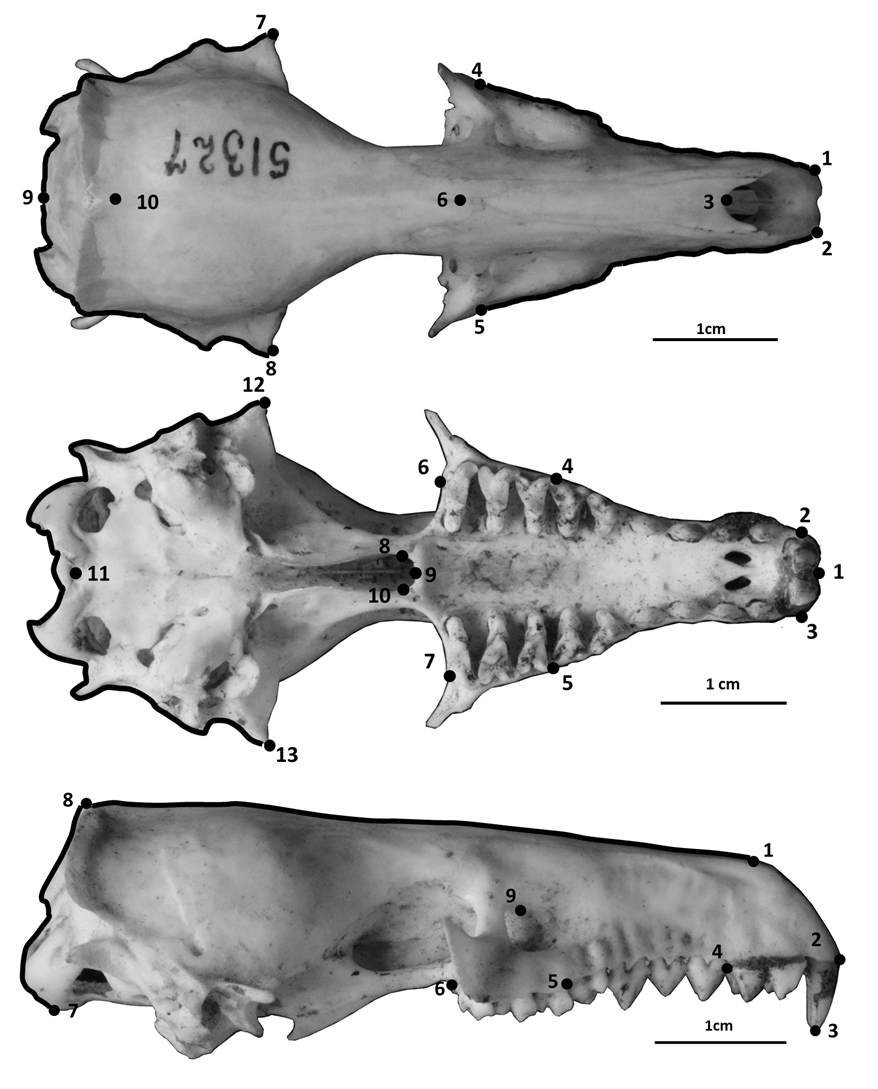
\includegraphics[width=1\linewidth]{figures/skdors+skvent+sklat_BW.png}
	
	\caption[Diagram of the landmarks and curves for the skulls in dorsal ventral and lateral views]
		{Landmarks (numbered points) and curves (black lines) used to capture the morphological shape of skulls in dorsal, ventral and lateral views respectively. Curves were re-sampled to the same number of evenly-spaced points. See Supplementary Material for descriptions of the curves and landmarks. The specimens belong to two different \textit{Potamogale velox} (Tenrecidae) skulls: accession number AMNH 51327 (dorsal) and BMNH 1934.6.16.2 (ventral and lateral)}
	
	\label{fig:skulls_landmarks}
	\end{figure}


%************************************************** 

	
%-------------------------------------------------------	
\subsection{Calculating morphological diversity}



	We calculated morphological diversity using the results of our principal components analyses. We selected the principal components axes which accounted for 95\% of the cumulative variation for each of our three skull analyses. These axes represent the dimensions of our morphospace (REF). We used the scores from the PC axes to compare cranial morphologies in two ways.
	
	First, we used non parametric MANOVAs \citep{Anderson2001} to test whether tenrecs and golden moles occupied significantly different positions within our cranial morphospaces \citep[e.g][]{Serb2011, Ruta2013}.
	Secondly, we compared morphological diversity within tenrecs to the diversity within golden moles. If tenrecs are more morphologically diverse, then they should be more spread-out within our cranial morphospaces. We calculated the morphological diversity of each Family as the mean Euclidean distance between every species and the centroid for that Family. We used a t test to assess whether there was any significant difference in the morphological diversity of tenrecs and golden moles.
	
	Our groups have unequal sample sizes (31 tenrec species compared to 12 golden mole species). Therefore, we could find higher morphological diversity in tenrecs simply because it is the larger group (REF). We used pairwise permutation tests to account for this potential bias in sample size. Our null hypothesis was that there is no difference in morphological diversity between tenrecs and golden moles. If this were true, then the group identity of each species would be arbitrary: if you randomly assign the species as being either a tenrec or golden moles and then re-calculate morphological diversity there would still be no difference between the two groups. 
	
	We assigned Family identities at random to each species and calculated the differences in morphological diversity (mean Euclidean distances to the Family's centroid) for the new groupings. We repeated these permutations 1000 times to generate a null distribution of the expected differences in morphological diversity between a group that has 31 members (tenrecs) compared to one which has 12 members (golden moles). Finally, we compared our observed (true) measures of the differences in morphological diversity to these permuted distributions to test whether there were significant differences in morphological diversity of the two Families after taking sample size differences into account.
	
	The majority of tenrec species (19 out of 31 in our dataset) are members of the \textit{Microgale} (shrew-like) Genus which is notable for its relatively low morphological diversity \citep{Soarimalala2011, Jenkins2003}. Therefore, the strong similarities among these species may mask signals of higher morphological diversity among other tenrecs. 
	To test this idea, we created a subset of our tenrec data which included
	just 5 of the \textit{Microgale} species. We compared the morphological diversity of this subset of tenrecs (n=19: 5 \textit{Microgale} with 12 other tenrec species) to the morphological diversity within the 12 species of golden moles. We repeated the same morphological diversity comparisons and permutation tests to account for differences in sample size on this reduced data set.
	 


% NC: Now this is shortened I'd stick the rarefaction in here too
	% SF: I took out rarefaction because Steve Wang and Steve Brusatte both advised that it was not the most appropriate test to use. The permutation method also takes sample size into account so I thought that removed the need for a rarefaction analysis aswell?
%-----------------------------------------------------------

\section{Results}
 
	%New axes numbers (select axes for 95 % of the variation, not one extra)
		%Full data: skdors =6, skvent=7, sklat =7
		%Microgale subset: skdors=6, skvent=6, sklat=6
	Figure \ref{fig:skdorsPCA} depicts the morphospace plot derived from our principal components analysis of average Procrustes-superimposed shape coordinates for skulls in dorsal view. Similar plots for our analyses of skulls in ventral and lateral views can be found in the supplementary material.
	To compare morphological diversity in the two families, we used the principal components axes which accounted for 95\% of the cumulative variation in each of our skull analyses: dorsal (n=6 axes), ventral (n=7 axes) and lateral (n=7 axes). 
	First, we compared the position of each Family within the morphospace plots. Tenrecs and golden moles occupy significantly different positions in the dorsal 	(npMANOVA, F \textsubscript{1,42} = 68.13, R$^2$ = 0.62, p=0.001 ), ventral (npMANOVA, F \textsubscript{1,42} = 103.33, R$^2$ = 0.72 , p=0.001 ) and lateral (npMANOVA, F \textsubscript{1,42} = 76.7, R$^2$=0.652, p=0.001 ) skull morphospaces,  indicating that the families have very different cranial morphologies. 
	%Numbers are from the npMANOVA based on PC axes within my diversity_twofamily_cent_dist script

	Secondly, we compared the morphological diversity within each Family. Based on our measures of mean Euclidean distances to the Family's centroid, tenrec crania are more morphologically diverse than golden mole crania in lateral view but not in dorsal or ventral view (table \ref{tab:diversity}). In contrast, when we compared morphological diversity within the sub-sample of 19 tenrecs (including just 5 \textit{Microgale} species) to the 12 golden mole species, we found that tenrecs had significantly higher cranial morphological diversity than golden moles in all analyses (table \ref{tab:diversity}).

	Our pairwise permutation tests for each analysis confirmed that (lack of) differences in morphological diversity were not artefacts of differences in sample size (see supplementary material).
		%Add the new permutation results to the supplementary
%************************************
%Results tables and figures
%Reduced it down to one table and one figure


	\begin{table}[h]			
	\caption[Comparison of morphological diversity in tenrecs and golden moles.]
	\centering{Morphological diveristy in tenrecs and golden moles for each of the three analyses (skulls in dorsal, ventral and lateral view). We measured morphological diversity as the mean Euclidean distance between each species and the centroid for their Family. We compared the morphological diversity of 12 species of golden mole to a) all 31 species of tenrec (left) and b) 19 species of tenrec (right) which included just 5 species of \textit{Microgale} tenrec. Significant differences (p values from t-test comparisons) are highlighted in bold.}
	%Diversity based on centroid distances results summary
%All tenrecs and golden moles
%Morphological diversity based on comparing the mean Euclidean distances to each family's centroid
%NB: degrees of freedom are different in each analysis because I'm using a Welch two sample t test: df comes from a distribution of values based on the error within each sample so the final numbers will be different for each data set

%Re-ordered the table so that everything would fit in better


\resizebox{\columnwidth}{!}{
%Scales down the table to fit within the column width
	% If this is too small then I'll probably need to break the table into two
\begin{tabular}{c l c c c c}		
\hline
N& Analysis & \multicolumn{2}{c}{Morphological diversity} & t\textsubscript{df} & p value\\
%-----------------------------------------------
\hline
%------------------------
 &  & Tenrecs  & Golden moles &  &  \\
%--------------------------------
\cline{3-4} % Puts a line just through some columns
%---------------------------------
 & & (mean $\pm$ s.e) & (mean $\pm$ s.e) & &\\
\hline
%\multicolumn{1}{l}
%---------------------------
 31 & Skulls dorsal & \multicolumn{1}{l}{0.036 $\pm$ 0.0029} & 0.029 $\pm$ 0.0032 & -1.63\textsubscript{29.88}& 0.11 \\
%--------------------------------------
 & Skulls ventral & \multicolumn{1}{l}{0.048 $\pm$ 0.0034} & 0.044 $\pm$ 0.0041 & -0.68\textsubscript{26.99} & 0.51\\
%-----------------------------------------
 & Skulls lateral & 0.044 $\pm$ 0.0041 & 0.032 $\pm$ 0.0037 & -2.16\textsubscript{35.03} & \textbf{0.04}\\
%----------------------------------------
 & Mandibles & 0.049 $\pm$ 0.0044 & 0.067 $\pm$ 0.0054 & 2.62\textsubscript{25.85} & \textbf{0.01}\\
%--------------------------
\hline
%-----------------------------------------
17 & Skulls dorsal & 0.044 $\pm$ 0.0025 & \multicolumn{1}{l}{0.029 $\pm$ 0.0032} & -3.62\textsubscript{22.75} & \textbf{<0.01}\\
%---------------------------------
 & Skulls ventral & \multicolumn{1}{l}{0.054 $\pm$ 0.0039} & \multicolumn{1}{l}{0.042 $\pm$ 0.0041} & -2.23\textsubscript{25.46} & \textbf{0.04}\\
%-------------------------------------
 & Skulls lateral &  \multicolumn{1}{l}{0.054 $\pm$ 0.0053} & 0.031 $\pm$ 0.0037 & -3.47\textsubscript{26.31} & \textbf{<0.01} \\
%--------------------
 & Mandibles & 0.055 $\pm$ 0.0049 & \multicolumn{1}{l}{0.062 $\pm$ 0.0050} & 1.00\textsubscript{25.88} & 0.33 \\
%--------------------

\hline
\end{tabular}
} 
	\label{tab:diversity}  
	\end{table}

		
%PCA figure: Just skdors as an example
	%From the diversity_twofamily_cent_dist script
	\begin{figure}[H]
	\centering
	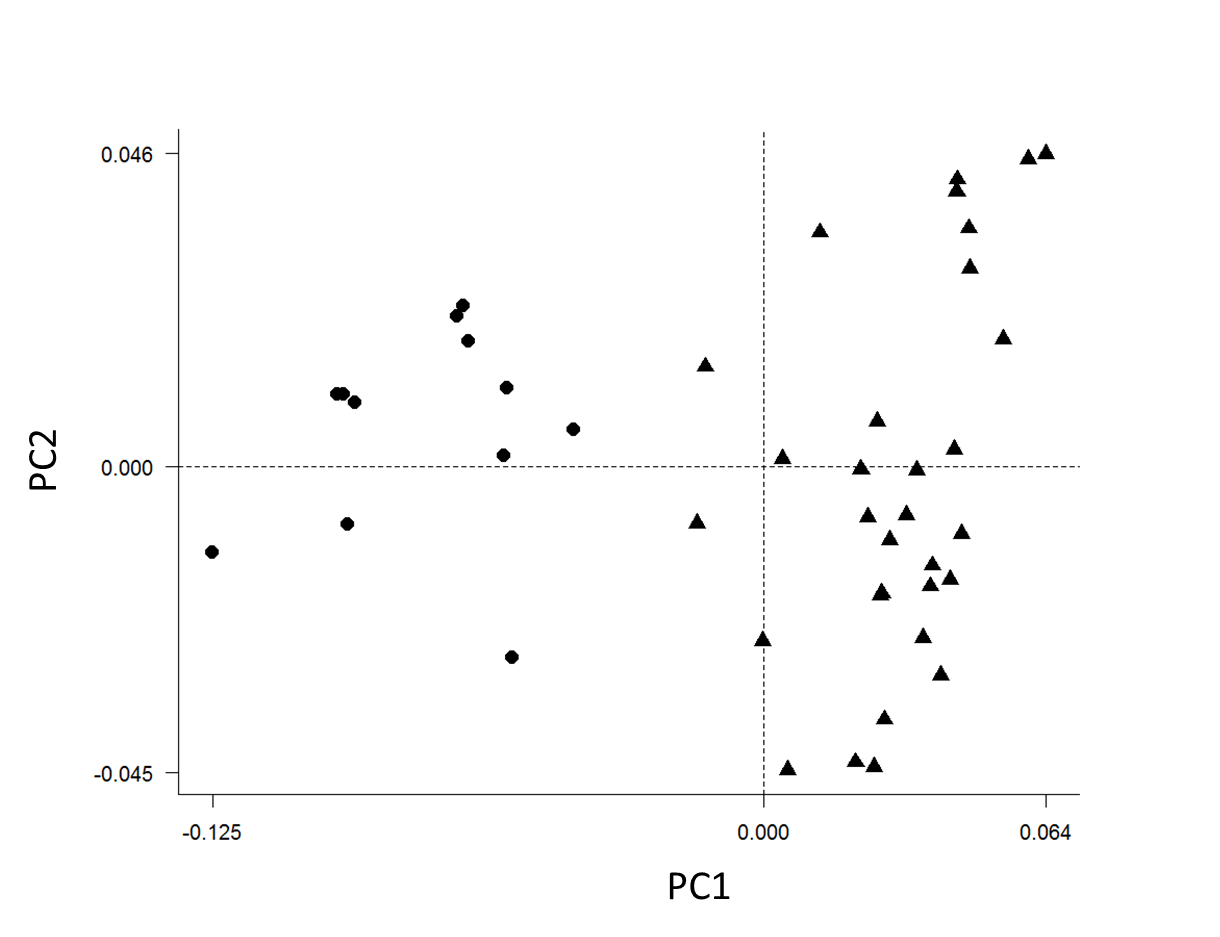
\includegraphics[width=1\linewidth]{figures/skdors_PCA_allspecies_BW.png}
	\caption[Morphospace (principal components) plot of morphological diversity in dorsal views of tenrec and golden mole skulls.]
		{Principal components plot of the morphospace occupied by tenrecs (triangles, n = 31 species) and golden moles (circles, n = 12) for the skulls in dorsal view. Axes are PC1 and PC2 of the average scores from a PCA analysis of mean Procrustes shape coordinates for each species. }
	\label{fig:skdorsPCA}
	\end{figure}
%**********************************************


\section{Discussion} 

% NC: OK this section needs another proper go over. I don't get what you're trying to say in most places. Worth going back to the intro and making sure you draw in all the themes you touch on there. So your concluding remarks should be about adaptive radiation. Try writing this discussion again, using the same techniques as for writing introductions. Except the direction is narrow to broad rather than broad to narrow. Have a reason for each paragraph, a story you want to tell.

%1) Specific discussion of results and differences between skulls and mandibles
	Our analyses are the first quantitative investigation of morphological disparity in tenrecs. We show that tenrecs' cranial morphologies are no more diverse than their closest relatives and therefore phenotypic variety in tenrecs is perhaps not as exceptional as it first appears.
	
	When we compared the diversity of skull shapes in the two Families, we found a trend towards higher disparity in tenrecs compared to golden moles but none of these differences were significant (table \ref{tab:disp.summary}). Even when we removed the phenotypically similar \textit{Microgale} Genus, tenrecs were still no more diverse than golden moles in most of the analyses of their skull shapes (table \ref{tab:disp.nonmic.summary}). 
	
	In contrast to these results for the skulls, two of our disparity metrics indicate that golden moles have more disparate mandible shapes than tenrecs (table \ref{tab:disp.summary}).
	We recognised that our landmarks and curves for the mandibles focus particular attention on the ascending ramus (condyloid, condylar and angular processes, figure \ref{fig:sklat_mands_landmarks}). Therefore we deleted the three semilandmark curves around these structures and repeated our disparity calculations. In this case we found no significant differences in disparity between the two Families (table \ref{tab:disp.summary}). Therefore, our results seem to indicate that golden moles have greater morphological variation in the posterior structures of their mandibles compared to tenrecs.
		
	%I asked for advice from Gary Bronner about why I was getting higher variation in golden mole mandibles compared to tenrecs. He thinks that the most likely reason is a problem with my landmarks. Landmark 4 is the alveolus of the last molar but that position is not homologous across species because of the presence/absence of a third molar. His advice was to re-run the analysis without landmark 4 and curve A and see what patterns of shape variation come out then.
		
	%However, as I was choosing the landmarks I knew that the dental formulae varied for each species - and therefore the landmarks are relative points showing the end of the tooth row rather than biologically meaningful positions of dental characteristics. But now I don't know if I can get away with using that as an excuse when it comes to trying to explain strange results in my paper.
			
	 Given that these posterior structures act as muscle attachment and articulation sites for connections with the upper jaw, %needs a ref ?
	 one might expect that golden moles with highly disparate posterior mandible morphologies should also show high variability in the corresponding mandible articulation areas of the skull. However, we could not locate reliable, homologous points accurately on those areas of the skull pictures in lateral view. Instead, our landmarks and semilandmark curves for the skulls in lateral view focus attention on morphological variation in the dentition and the overall shape of the top and back of the skulls (figure \ref{fig:sklat_mands_landmarks}). This may explain why golden mole skulls in lateral view do not show the same pattern of higher disparity compared to tenrecs that we see in our analyses of the mandibles. However, further investigation is required to identify possible reasons why golden moles appear to show such variation in the posterior structures of their mandibles.
	 	%SF: I know this is a weak ending but I'm still figuring out possible reasons for this pattern that aren't just data problems. 
	 	
		%The discrepancies could arise from factors associated with the modularity of morphological evolution.
	
		%There is strong evidence that morphological variation in skulls and mandibles is derived from differential evolution of integrated developmental modules \citep[reviewed by][]{Klingenberg2013a}.
		%For example, there seems to be two primary modules in the mouse mandible; an alveolar part which holds the teeth and the ascending ramus for muscle attachment and which articulates with the skull \citep{Klingenberg2008a}. Geometric shape covariation is stronger within rather than between these modules. 
	
	% NC: I don't really get the relevance of this part...
	% SF: It was just one of my ideas for trying to figure out why I'm getting different patterns in the mandibles compared to the skulls but I didn't manage to develop it properly
	
%------------------------------------------------------	
%2) Skulls are only one way of looking at diversity but it's still interesting to see that ecologically diverse tenrecs are no more disparate than the functionally similar golden mole family
	
	We used variation in skull and mandible shapes as proxy measures for overall morphological diversity within the two Families. Many other studies also use skulls to study phenotypic variation within species \citep{Blagojevic2011, Bornholdt2008}, to delineate species boundaries within a clade \citep[e.g.][]{Panchetti2008} or for cross-taxonomic comparative studies of phenotypic (dis)similarities \citep[e.g.][]{Ruta2013, Goswami2011, Wroe2007}.
	
	However, studies of morphological disparity are inevitably constrained to measure diversity within specific traits rather than overall phenotypes \citep{Roy1997}. Disparity calculations based on skull shape can yield similar results compared to analyses of whole-skeleton discrete characters and limb proportion data sets \citep{Foth2012}. Yet it is still possible that comparing disparity in tenrecs and golden moles using non-cranial morphological measures could produce different results. For example, tenrecs inhabit a wide variety of ecological niches and habitats including terrestrial, arboreal, semi-aquatic and semi-fossorial environments \citep{Soarimalala2011}. In contrast, although golden moles occupy a wide altitudinal, climatic and vegetational spectrum of habitats \citep{Bronner1995}, they are are all fossorial species which, superficially at least, appear to be less functionally diverse than tenrecs. Therefore, comparing the disparity of limb morphologies within the two Families could indicate that tenrecs are more morphologically diverse than golden moles and therefore support the claim that tenrecs are an exceptionally diverse group. 
	
	
%------------------------------------------
%Wider relevance to adaptive radiation

 	Our analyses are the first measures of morphological diversity within tenrecs, a group which is commonly cited as an example of an adaptive radiation \citep{Olson2013}. Evidence of exceptional morphological diversity is one criterion for designating a clade as an adaptive radiation \citep{Losos2010a}. However, we found that tenrecs are no more morphologically diverse than their their closest relatives and therefore, within our tests, do not appear to show the exceptional diversity which characterises an adaptively radiated group.   
 	
 	The evolution of cranial shape (both upper skull and mandible), particularly dental morphology, has obvious correlations with dietary specialisations and occupation of specific ecological niches \citep[e.g.][]{Wroe2007}. Considering the wide ecological diversity of the tenrec Family; semi-fossorial, arboreal, terrestrial and semi-aquatic \citep{Soarimalala2011}, we think that it is reasonable to expect that this variety should be reflected in skull morphology. However, we have not included any measures of the `adaptiveness' of cranial shape in our analyses and therefore our analyses should not be considered to be an explicit test of whether or not tenrecs are an adaptive radiation \citep{Losos2010a}. Instead we have made the first step towards understanding the apparent phenotypic diversity within tenrecs within a quantitative framework. Future work should focus on explicit measures of the `adaptiveness' and functional importance of tenrec cranial and post-cranial morphologies to understand the significance of morphological diversity within the Family \citep[e.g.][]{Mahler2010}. However, we also recognise that strict, statistically based categorisations of clades as being adaptive radiations or not are not always biologically meaningful or helpful when it comes to trying to understand patterns of phenotypic diversity \citep{Olson2009}.   


%---------------------------------------------------	
%4) Conclusions
	We have presented the first quantitative study which tests the common claim that tenrecs are an exceptionally diverse group \citep{Olson2013, Soarimalala2011,Eisenberg1969}. Focusing on cranial diversity is only one aspect of morphological variation and further analyses are required to test whether other morphological traits yield similar patterns. However, our results provide a clear indication that phenotypic variety within tenrecs is perhaps not as exceptional as it first seems.   
	
\section{Acknowledgements}

	We thank Fran\c{c}ois Gould, Dean Adams, David Polly, Gary Bronner, Steve Brusatte, Steve Wang, Luke Harmon, Thomas Guillerme and the members of NERD club for insightful discussions and the museum staff and curators for their support and access to collections. Funding was provided by an Irish Research Council EMBARK Initiative Postgraduate Scholarship (SF) and the European Commission CORDIS Seventh Framework Programme (FP7) Marie Curie CIG grant. Proposal number: 321696 (NC)

\bibliographystyle{jeb}
\bibliography{refs_disparity}
% I downloaded the jeb.bst file from http://schneider.ncifcrf.gov/latex.html but there isn't an associated style file

% NC: You can make one via the command line as I showed you in one of my LaTeX lessons.

	%**********************
	%SF: I still need to do this so that the references have the abbreviated journal titles, don't include the doi and so that book references don't have the total number of pages but do have the editors' names
	%*******************************************




\end{document}